\documentclass[aspectratio=43]{beamer}
\usepackage[utf8]{inputenc}


%%%%%%%%%%%%%%%%%%%%%%%% THEME
\usetheme{material}
\useLightTheme
\usePrimaryGreen
\useAccentRed

\usepackage{macros} % must come after theme

\title{\q Factorization}
\keywords{\qc, \q Factorization, Shor's algorithm, Cryptography}

\begin{document}

\begin{frame}
	\titlepage
\end{frame}


\begin{frame}{Table of contents}
	\begin{card}
		\tableofcontents
	\end{card}
\end{frame}


\section{Introduction}
\begin{frame}{Introduction}
    \begin{card}
        This week is dedicated to studying the quantum algorithm that, arguably, has had the most \textbf{astonishing impact} insofar on the world and it helped raise interest in \qc and reach nowadays \textbf{quantum's critical mass}!
    \end{card}
    \begin{card}
        \textit{Unlike} other quantum algorithms that we have studied, this one is named after its creator: \href{https://en.wikipedia.org/wiki/Peter_Shor}{Peter Shor} (\textbf{\sa}). It brings an \textbf{exponential speed-up} on a very important problem nowadays: \textbf{prime factorization}.
    \end{card}
\pagenumber
\end{frame}
\begin{frame}{Introduction}
    \begin{card}
        So, we will understand \textbf{which} problem \sa solves and \textbf{how} it does so. However, we do not want an \textit{exponential speed-up} in the complexity of this course and so, some of the mathematical concepts will be concealed and you will have a chance to study it both in the week's exercise as well as in the recommended links at the end.
    \end{card}
\pagenumber
\end{frame}


\section{Prime Factorization problem}
\begin{frame}{Prime Factorization problem}
    \begin{card}
        Given a number $N$ we would like to find a pair of prime numbers ($p$, $q$) whose product equals $N$: $p\times q=N$. The existence of this pair is \textbf{guaranteed} by the \href{https://en.wikipedia.org/wiki/Fundamental_theorem_of_arithmetic}{fundamental theorem of arithmetic}.
    \end{card}
    \begin{card}
        Algorithms for achieving this already exist, however this problem fits into the \np family and is computationally possible only for small values of $N$, as nowadays \textbf{classical} computers are unable to find it in feasible time.
    \end{card}
\pagenumber
\end{frame}



\section{Cryptography considerations}
\begin{frame}{Cryptography considerations}
    \begin{card}
        The opposite process, finding large primes is relatively easy (\href{https://en.wikipedia.org/wiki/Primality_test}{primality test} or \href{https://en.wikipedia.org/wiki/Sieve_of_Eratosthenes}{Sieve of Eratosthenes}) and multiplying them as well.
    \end{card}
    \begin{card}
        As such, many \href{https://en.wikipedia.org/wiki/Public-key_cryptography}{cryptography} algorithms rely on that easiness and on the factorization hardness to provide a secure means of communication. If this still seems odd, lets just say that the trustworthiness of most requests made from your browser to online servers rely on it, not to mention innumerable encryption mechanisms out there.
    \end{card}
\pagenumber
\end{frame}

\section{\sa}
\begin{frame}{\sa \ Overview}
    \begin{cardTiny}
        It would be a true hindrance if prime factorization were to become a \textbf{feasible problem}. The world would have to be redefined from scratch and countless consequences on data privacy and safety would arise, of \textbf{unimaginable proportions}.
    \end{cardTiny}
    \begin{cardTiny}
        As a matter of fact, that is what Peter Schor has done (and his name definitely belongs on the algorithm) for the only thing preventing this catastrophic event is that real quantum computers are still a few steps short of allowing for such complex computations. One might say: \textit{thankfully we found the \textbf{theory before the technology} arrived.}
    \end{cardTiny}
\pagenumber
\end{frame}

\begin{frame}{\sa Overview}
    \begin{card}
        Technically speaking, \sa solves prime factorization through the following steps:
        
        \begin{enumerate}
            \item Formulation of prime factorization as a period finding problem
            \item Quantum algorithm to solve period finding
            \item Conversion of period back into prime factors
        \end{enumerate}
        
        We will go over each of these, but the heart of the speed-up lies in the quantum algorithm in question: \textbf{\qft}
    \end{card}
\pagenumber
\end{frame}

\begin{frame}{\sa Overview}
    \begin{card}
        \begin{center}
            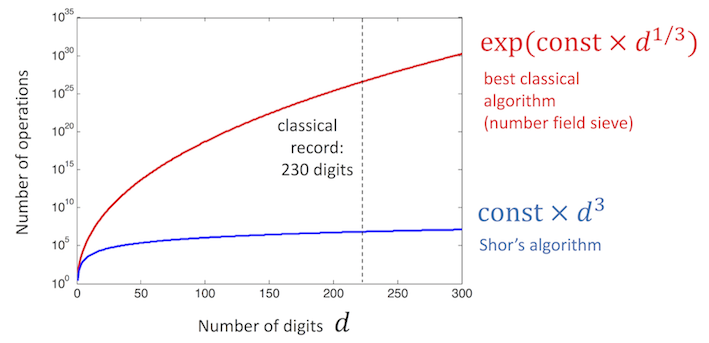
\includegraphics[width=1\textwidth]{factorization_speed}
        \end{center}
    \end{card}
\pagenumber
\end{frame}


\subsection{From Factorization to Period Finding}
\begin{frame}{From Factorization to Period Finding}
    \begin{card}
        The first trick of this endeavour was to discover that if we want to factorize $N$, we can start by the fact that:
        \begin{equation*}
            f(a) = x^a \mod N^*
        \end{equation*}
        is a \textbf{periodic} function, where $x$ is \href{https://en.wikipedia.org/wiki/Coprime_integers}{coprime} with $N$ and $a \geqslant 0$
    \end{card}
    \begin{card}
        *If necessary, review the \href{https://www.khanacademy.org/computing/computer-science/cryptography/modarithmetic/a/what-is-modular-arithmetic}{mod operator}.
    \end{card}
\pagenumber
\end{frame}

\begin{frame}{From Factorization to Period Finding}
    \begin{card}
        Since $f(a)$ is periodic, it follows that there is a period \textbf{r}:
        \begin{equation*}
            (x^0 \mod N = 1) \Rightarrow (x^r \mod N = 1)
        \end{equation*}
        Since $x^0=1$, and considering the periodic nature of $f$, which grows from $a=0$ to $a=r$.
    \end{card}
    \begin{card}
        At this stage, let us focus on how the discovery of \textbf{r} can be achieved \textit{quantumly}. We will go back to this formulation once we know the period.
    \end{card}
\pagenumber
\end{frame}

\subsection{\qft}
\begin{frame}{\qft}
    \begin{card}
        The secret behind the exponential speed-up lies at this stage of the algorithm - \qft. This is an operation analog to that of the \href{https://en.wikipedia.org/wiki/Discrete_Fourier_transform}{Discrete Fourier Transform}. Unlike the classical version, the \qft can be implemented on $O(n^2)$ (polynomial) gates, whereas the classical version would require $> O(2^n)$ (exponential).
    \end{card}
    \begin{card}
        The \qft can be constructed using only Hadamard ($H$) and phase shift ($R_{\phi}$) gates!
    \end{card}
\pagenumber
\end{frame}

\begin{frame}{\qft}
    \begin{card}
        We will get to implement it on this week's exercises. Suffice to say, for now, that it achieves the task of uncovering \textbf{r} \textbf{exponentially faster} than in classical systems, by making use of quantum \textbf{superposition} to test multiple values at once. 
    \end{card}
    \begin{card}
        It should be noted that the underlying math is advanced and would make little sense to include it here, due to its level of specificity. You are, however, expected to understand the high-level mechanism behind the algorithm and, with time, you may feel the need to study it thoroughly.
    \end{card}
\pagenumber
\end{frame}


\newcommand{\xrsq}{x^{\frac{r}{2}}}
\newcommand{\pxrsq}{(\xrsq + 1)(\xrsq - 1)}
\subsection{From Period to Factors}
\begin{frame}{From Period to Factors}
    \begin{card}
        After \textbf{r} is found, we now need to go back to our modular arithmetic and perform the following manipulation:
        \begin{equation*}\begin{split}
            x^r \equiv 1 \mod N \Leftrightarrow \\ 
            (\xrsq)^2 \equiv 1 \mod N \Leftrightarrow \\
            (\xrsq)^2 - 1 \equiv 0 \mod N  \Leftrightarrow \\
            \pxrsq \equiv 0 \mod N \text{(even $r$)}
        \end{split}\end{equation*}
        Notice that $\pxrsq$ is a multiple of $N$. So long as at least one of those factors is not a multiple of $N$ then it has a common divisor with $N$.
    \end{card}
\pagenumber
\end{frame}

\begin{frame}{From Period to Factors}
    \begin{card}
        Thus, we need only compute the \href{https://en.wikipedia.org/wiki/Greatest_common_divisor}{greatest common divisor} (gcd) between $N$ and each of $(\xrsq + 1)$ and $(\xrsq - 1)$:
        \begin{equation*}
            gcd(N, \xrsq + 1) = PossibleFactor1
        \end{equation*}
        \begin{equation*}
            gcd(N, \xrsq - 1) = PossibleFactor2
        \end{equation*}
        The $gcd$ can be calculated in \textbf{polynomial time} using an algorithm that was described more than 2300 years ago by Euclides, the \href{https://en.wikipedia.org/wiki/Euclidean_algorithm}{euclidean algorithm}. 
    \end{card}
\pagenumber
\end{frame}

\section{\sa's considerations}
\begin{frame}{\sa's considerations}
    \begin{card}
        \sa's power is still limited by today's quantum computers (which can have in the order of 50 to 70 \textit{good quality} qubits) and it can only be used to factor very small numbers (that you could factor by hand).
    \end{card}
\pagenumber
\end{frame}

\begin{frame}{\sa's considerations}
    \begin{card}
        To make \sa a security threat on today's world, one would need at least a couple thousand \textit{good quality} qubits, which is still a few years away (one can only hope). There is time and plenty of ideas like that of \q Cryptography (the quantum equivalent of typical cryptography) which will prevent many catastrophes to happen, hopefully!
    \end{card}
\pagenumber
\end{frame}

\section{Hands-on}
\begin{frame}{Hands-on}
    \begin{card}
        In this lesson, you have been given the logic behind \sa and you should have a good grasp of its impact. This week, there will be two practical exercises: one on \qft and another on \sa (which also mentions \qft). Both provide a more in-depth description of the underlying math (don't worry if it is to overwhelming, you can build on that knowledge) and also a walk-through using \qk of the implementation of \sa.
    \end{card}
\pagenumber
\end{frame}




\section{Where to learn more?}
\begin{frame}{Where to learn more?}
\begin{card}
    \begin{itemize}
        \item \href{https://arxiv.org/abs/quant-ph/9508027}{Original Paper by Peter Shor}
        \item \href{https://www.youtube.com/watch?v=hOlOY7NyMfs}{Peter Shor} a very short video of the man, the myth, the legend on his algorithm
        \item \href{https://quantumexperience.ng.bluemix.net/proxy/tutorial/full-user-guide/004-Quantum_Algorithms/110-Shor's_algorithm.html}{Tutorial from \ibmqe} on \sa
        \item \href{http://www-math.mit.edu/~shor/GRRM-poetry.html}{Shor's poetry on Game of Thrones} (for when you feel tired)
    \end{itemize}
\end{card}
\end{frame}
\end{document}
